\documentclass[conference, 10pt]{IEEEtran}
\usepackage[cmex10]{amsmath}
\usepackage{amssymb}
\usepackage{graphicx}
\usepackage{color}
\usepackage{placeins}
\usepackage{bm}
\usepackage{cite}
%\usepackage{stfloats}
\usepackage{float}
\usepackage{hyperref}
\usepackage{cite}
\usepackage{tabularx,colortbl}
\DeclareMathOperator*{\argmin}{arg\,min}

\begin{document}
\title{\texttt{maoud}: a Python package for Simulating Generalized Fading Channels}

\author{\IEEEauthorblockN{Jos\'e~V.~de~M.~Cardoso,~Wamberto~J.~L.~Queiroz,}
        \IEEEauthorblockN{~Paulo~R.~Lins~J\'unior,~and~Marcelo~S.~Alencar,~\textit{IEEE Senior Member}}
\IEEEauthorblockA{Universidade Federal de Campina Grande\\
Instituto Federal de Educa\c c\~ao, Ciencia, e Tecnologia da Para\'iba\\
Campina Grande, Para\'iba, Brasil\\
\{josevinicius, wamberto, paulo, malencar\}@iecom.org.br\\}
}

\maketitle

\begin{abstract}
    We present a well tested Python-based library for simulating and computing
    generalized fading channels, named \texttt{maoud}. We describe the
    applicability of \texttt{maoud} using examples in scenarios of communications
    channels impaired by generalized fading, namely: spectrum sensing, bit error
    rate computation, and fading estimation. For the latter, we develop an iterative
    algorithm using the Majorization-Minimization framework, which allows reliable
    estimation of the fading parameter. The development of \texttt{maoud} is open
    source and its code, along with the code for the examples presented in this
    paper, are avaliable at \texttt{http://github.com/mirca/maoud}.
\end{abstract}

\IEEEpeerreviewmaketitle
\section{Introduction}

The study of modern wireless communications systems heavily relies on fading channel simulation.
By fading channel simulation, we refer to the generation of samples from a probability distribution
that resembles the effects and impairments caused by real communications fading channels on the
transmitted signal.

Although accurate and precise distributions for generalized fading have been
estabilished in the literature, such as $\alpha\text{-}\mu$~\cite{yacoub.2007.1},
$\kappa\text{-}\mu$~\cite{yacoub.2007.2} and $\eta\text{-}\mu$~\cite{yacoub.2007.2},
the generation of samples following these distributions is usually
a time-consuming task. In~\cite{cogliatti2012}, the authors built an efficient
algorithm, based on the rejection method, for generation of samples from those
distributions.


however, there are neither open nor
closed source implementations available to the scientific community.

In this paper, we present an open source Python package, named \texttt{maoud},
for generation of samples following the $\alpha\text{-}\mu$, $\kappa\text{-}\mu$, and
$\eta\text{-}\mu$ distributions. The usefullness of $\texttt{maoud}$ is illustrated
through examples involving spectrum sensing, bit error rate (BER) computation, and
fading estimation.

\subsection*{Notation}
Scalars and random variables are denoted as italic, small-case letters
\textit{e.g.} $x$; sets and events are denoted as italic, capital
letters \textit{e.g.}, $A$; vectors and random vectors are denoted as
italic, boldface, small-case letters \textit{e.g.} $\bm{x}$. The $n-$th
component of a vector $\bm{x}$ is denoted as $x_n$. A complex vector of length
$n$ is defined as $\bm{x} \in \mathbb{C}^{n\times 1}$. All vectors are column
vectors. Matrices are denoted as italic, boldface, capital letters as
in $\bm{X}$; the identity matrix of order $n$ is denoted as $\bm{I}_n$. We
define a discrete-time circularly symmetric Gaussian process $\bm{z}$ as any
collection of random variables $\bm{z}~=~\bm{x}~+~j\bm{y}$,
$j \triangleq \sqrt{-1}$, such that $\bm{x}$ and $\bm{y}$ are i.i.d. jointly
Gaussian, with zero mean vector and covariance matrix given by
$\mathbb{E}\left(\bm{z}\bm{z}^{\dagger}\right)$, in which $\bm{z}^\dagger$ means
the conjugate transpose of $\bm{z}$. The expectation value with respect to the
probability distribution of a random variable $x$ is denoted as $\mathbb{E}_x$.
The probability of an event $A$ is denoted as $\mathbb{P}(A)$. The indicator
function is denoted as $\mathbb{I}(\cdot)$, it evaluates to one if its argument
is true and zero otherwise. For any given two real functions $f$ and $g$ defined
on the same domain $D$, $f \cong g$ means that there exist a constant $c$ such that
$f(\bm{x}) = g(\bm{x}) + c$, $\forall~ \bm{x} \in D$. The natural logarithm of a
scalar $x > 0$ is denoted as $\log x$.

\section{Rejection sampling}

\section{Examples}
\subsection{Spectrum Sensing in Complex Generalized Fading Channels}

The spectrum sensing problem consists in deciding whether or not a given channel
frequency band is being occupied by a licensed (primary) user and, in case that such
frequency band is available, how to opportuniscally allocate secondary users
such that the interference on the primary user is negligible.

From a probabilistic point of view, the spectrum sensing problem may be framed as
a decision theory problem, as follows
\begin{align}
    H_0:~& \bm{y} = \bm{w},\\
    H_1:~& \bm{y} = h\bm{s} + \bm{w},
\end{align}
in which $\bm{y} \in \mathbb{C}^{n\times 1}$ is the received vector signal,
$\bm{w} \in \mathbb{C}^{n\times 1}$ is complex Gaussian noise process with zero mean
vector and covariance matrix given as $\sigma^2\bm{I}_n$, and $h$ is the channel gain.

In~\cite{cardoso2017}, the authors have shown that the cumulative distribution function (cdf) of the
energy statistic $\tilde{y} \triangleq \bm{y}^{\dagger}\bm{y}$ conditioned on the knowledge of $h$,
in case that $\bm{s}$ is an $M$-PSK signal such that every symbol has the same probability of occurrence,
$\mathbb{P}(s_n = s) = \frac{1}{M}$, is given as
\begin{align}
    P(\tilde{y} | h, H_1) = 1 - \mathrm{Q}_{n}\left(\sqrt{\dfrac{2n|h|^2E_s}{\sigma^2}}, \sqrt{\dfrac{2\tilde{y}}{\sigma^2}}\right),
\end{align}
in which $\mathrm{Q}_{n}$ is the Marcum-$\mathrm{Q}$ function and $E_s$ is the energy per symbol.

Recall that the energy detection rule can be expressed as
\begin{equation}
    d_\delta (\tilde{y}) = \mathbb{I}(\tilde{y} > \delta)
\end{equation}
in which $\delta$ is a strictly positive real number known as energy threshold,
and $d_\delta (\tilde{y}) = j,~j \in \{0,1\}$, means that the detector has decided
in favor of the hypothesis $H_j$.

As a result, the probabilities of false alarm and miss detection can
be written as
\begin{align}
    \mathbb{P}\left(d_\delta(\tilde{y}) = 1 | H_0\right) &=
        1 -  P(\delta | H_0) = 1 - \gamma\left(n, \frac{\delta}{\sigma^2}\right),\label{eq:pf} \\
    \mathbb{P}\left(d_\delta(\tilde{y}) = 0 | H_1\right) &= \mathbb{E}_{h}\left(P(\delta| h, H_1)\right)\nonumber\\
    &= \int_{-\infty}^{+\infty} P(\delta | h, H_1)p(h)\;\mathrm{d}h,\label{eq:pd}
\end{align}
in which $\gamma$ is the regularized lower incomplete Gamma function, $p(h)$ is the pdf of the fading,
and $\delta$ is the energy detection threshold.

The performance of detection schemes can be measured by computing the Receiver Operating
Characteristic (ROC), which consists in varying $\delta$ and computing the pairs of
probability of false alarm and miss detection, as illustrated in Fig.~\ref{fig:spectrum-sensing}.

\begin{figure}[!htb]
    \centering
    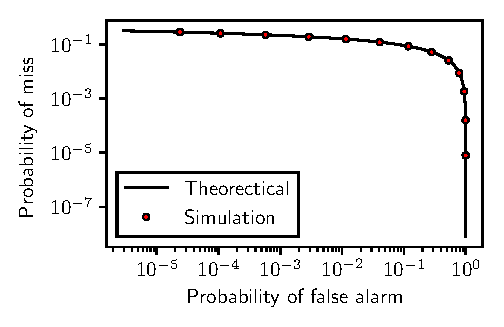
\includegraphics{figures/spectrum_sensing.eps}
    \caption{Receiver Operating Characteristic for the energy detector in $\alpha$-$\mu$
             fading channel with $\alpha=2$ and $\mu=1$, i.e., Nakagami-$m$, $m = 1$.
             The solid curve represents the theorectical probabilities as stated on
             (\ref{eq:pf}) and (\ref{eq:pd}) for different values of
             $\delta$, whereas bullets represent Monte Carlo simulations acquired with $10^6$ realizations.
             The input signal $\bm{s}$ consists in a vector of length $n=25$ in which each entry represents
             a symbol of a 64-PSK constellation. Symbols are assumed to be equiprobable.
             The signal-to-noise ratio is set to $5$ dB.}
    \label{fig:spectrum-sensing}
\end{figure}

\subsection{Parameter Estimation in Nakagami-$m$ fading}
The Nakagami-$m$ density is given as
\begin{align}
    p(\bm{h} &| m) = \prod_{i=1}^{n}\dfrac{2m^m}{\Gamma(m)\Omega^{m}}h_i^{2m - 1}
              \exp\left(-\dfrac{mh_i^2}{\Omega}\right) \nonumber \\
          = & \left(\dfrac{2m^m}{\Gamma(m)\Omega^{m}}\right)^{n}
          \exp\left(-\dfrac{m\sum_{i=1}^{n}h_i^2}{\Omega}\right) \prod_{i=1}^{n}h_i^{2m - 1},
\end{align}
in which $m$ is the fading parameter and $\Omega = \mathbb{E}(h_i^2)$ is the scale parameter.

The negative log-likelihood function (up to an additive constant) is given as
\begin{align}
-\log p(\bm{h} | m) \cong &-n\left(m\left(\log m - \log\Omega\right) - \log\Gamma(m)\right)\nonumber
    \\ & +m\sum_{i=1}^{n}\left(\dfrac{h_i^2}{\Omega} - 2\log h_i\right).
    \label{eq:loglike}
\end{align}

A direct maximum likelihood estimator (MLE) for (\ref{eq:loglike}) has been
shown to be infeasible~\cite{cheng2001}. Thus, we use the
Majorization-Minimization technique~\cite{sun2016} to find smooth
and easy to optimize upper bounds for $-\log p(\bm{h}| m)$.

Basically, the Majorization-Minimization (MM) algorithm consists in constructing a
sequence of functions $g(\cdot | m_t)$, initiliazed at $m_0$, such that
\begin{align}
    g(m | m_t) &\geq -\log p(\bm{h}| m) + c_t\label{eq:majorization-step},\\
    c_t &= g(m_t | m_t) + \log p(\bm{h}| m)\label{eq:mid-step},\\
    m_{t+1} &\in \argmin_{m > \frac{1}{2}} g(m | m_t)\label{eq:minimization-step}.
\end{align}
Note that (\ref{eq:majorization-step}) is the majorization step and (\ref{eq:minimization-step})
is the minimization step, whereas (\ref{eq:mid-step}) is a condition to ensure that the difference
of $g(\cdot | m_t)$ and $-\log p(\bm{h}| \cdot)$ is minimized at $m_t$.

Therefore, one possible way to construct $g(\cdot|m_t)$ is to find upper bounds for
$-m\log m$ and $\log \Gamma(m)$ for $m \geq \frac{1}{2}$.
The former function is concave for $m \geq 0$, hence it can be upper bounded
by its first order Taylor series as
\begin{align}
    -m \log m \leq -m(1 + \log m_t) + m_t,
    \label{eq:upper-bound-mlogm}
\end{align}
The function $\log \Gamma(m)$ is convex for $m > 0$, therefore, it can be upper bounded
by its second order Taylor series expansion as
\begin{align}
    \log \Gamma(m) \leq&  \log \Gamma(m_t) + \psi(m_t) (m - m_t)\nonumber\\
                        &  + \frac{\psi'\left(\frac{1}{2}\right)}{2}(m - m_t) ^ 2,
    \label{eq:upper-bound-negloggamma}
\end{align}
in which $\psi(x) = \dfrac{\Gamma'(x)}{\Gamma(x)}$ is known as the digamma function.
For both inequalities presented above, equality is achieved at $m = m_t$.

Applying inequalities (\ref{eq:upper-bound-mlogm}) and (\ref{eq:upper-bound-negloggamma}) into
(\ref{eq:loglike}), an upper bound for $\log p(\bm{h})$ is obtained as follows
\begin{align}
    &g(m | m_t) = - n\left.\Bigg[-m\log\Omega  + m(1 + \log m_t) - m_t\right.\nonumber\\
    & -\log \Gamma(m_t) - \psi(m_t) (m - m_t) \left. - \frac{\psi'\left(\frac{1}{2}\right)}{2}(m - m_t)^2\right]\nonumber\\
    & +m\left(\dfrac{\sum_{i=1}^{n}h_i^2}{\Omega} - 2\sum_{i=1}^{n}\log h_i\right)
    \label{eq:surrogate}
\end{align}

Due to the simple form of $g(m | m_t)$, its minimizer can be found in closed form, and
an updating rule for the MLE can be written as
\begin{align}
    m_{t+1} = m_t + \dfrac{1}{\psi'(\frac{1}{2})}&\left.\Bigg(1 + \log \frac{m_t}{\Omega} - \psi(m_t) \right.\nonumber\\
    &\left.+ \dfrac{1}{n} \sum_{i=1}^{n}\left(2\log h_i - \frac{h_i^2}{\Omega}\right)\right).
\end{align}

Additionally,
note that $\left\{m_{t+1}\right\}_{t \in \mathbb{N}}$ is a sequence of
estimators that converges to the MLE of the parameter value $m$. This
fact is a consequence of the convergence properties of the MM algorithm~\cite{sun2016}.
Therefore, the proposed estimator is asymptotically consistent and efficient.

We experimentally note, and it is also illustrated in Fig~\ref{fig:mm-example}, that the
estimator takes on average 30 iterations to converge within an absolute tolerance of $10^{-4}$.
\begin{figure}[!htb]
    \centering
    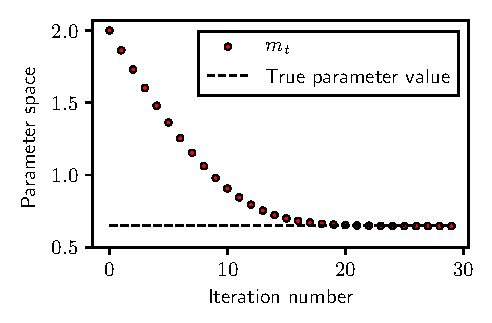
\includegraphics{figures/mm.eps}
    \caption{Typical convergence behavior of the proposed estimator.}
    \label{fig:mm-example}
\end{figure}

Moreover, we perform an experimental analysis of the bias and variance of the proposed estimator.
First, we recall that the Cram\'er-Rao Lower Bound for any unbiased estimator of $m$, say $\hat{m}$,
is given as~\cite{cheng2001}
\begin{align}
    \mathrm{var}(\hat{m}) \geq \dfrac{1}{n\left(\psi'(m) - \frac{1}{m}\right)}.
\end{align}


\begin{figure}[!htb]
    \centering
    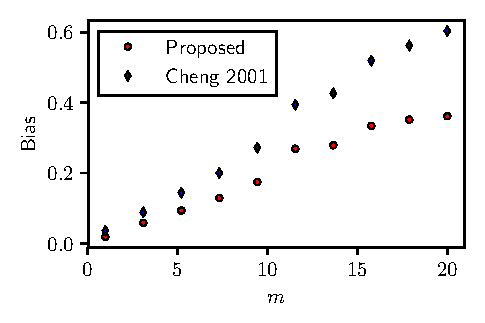
\includegraphics{figures/bias_N100.eps}
    \caption{Bias of the proposed estimator and the estimator presented in~\cite{cheng2001}.
             The bias was computed via Monte Carlo simulation with $10^4$ realizations.}
    \label{fig:bias}
\end{figure}

\begin{figure}[!htb]
    \centering
    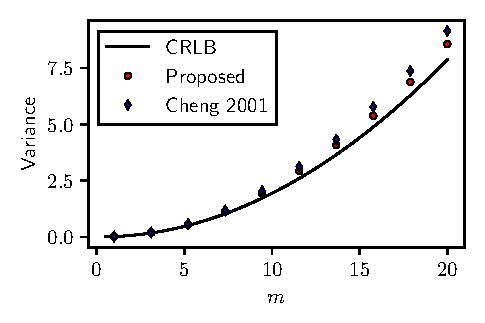
\includegraphics{figures/variance_N100.eps}
    \caption{Variance of the proposed estimator and the estimator presented in~\cite{cheng2001}
             compared against the Cram\'er-Rao Lower Bound. The variance was computed via
             Monte Carlo simulation with $10^4$ realizations.}
    \label{fig:variance}
\end{figure}

%Moreover, the expected value of $m_{t+1}$, conditioned on the knowledge of $m_t$, is given as
%\begin{align}
%    \mathbb{E}(m_{t+1} | m_t) = m_t + \dfrac{1}{\psi'(\frac{1}{2})}\left(\log \frac{m_t}{m} + \psi(m) - \psi(m_t)\right),
%\end{align}
%in which we used the fact that~\cite{gradshteyn2007}
%\begin{align}
%    \mathbb{E}\left(\log h_i\right)~=~\frac{1}{2}\left(\psi(m)-\log\left(\frac{m}{\Omega}\right)\right).
%\end{align}
%
%Most importantly, as $m_t \rightarrow m_{MLE}$ (due to convergence property of MM),
%then $\mathbb{E}(m_{t+1} | m_t) \rightarrow m_{MLE}$.
%
%The variance of $m_{t+1}$, given $m_t$, can be expressed as
%\begin{align}
%    \mathrm{var}(m_{t+1} | m_t) = \dfrac{\psi'(m) - \frac{1}{m}}{n\left(\psi'(\frac{1}{2})\right)^2}
%\end{align}
%
%\begin{align}
%    \mathbb{E}\left(\log ^ 2 h_1\right) &= \frac{1}{4}\left\{\left[\psi(m) - \log\frac{m}{\Omega}\right]^2 + \psi'(m)\right\}\\
%    \mathbb{E}\left(h_1^2\log h_1\right) &= \frac{\Omega}{2}\left(\psi(m+1) - \log\frac{m}{\Omega}\right)\\
%    \mathbb{E}\left(h_1^2\right) &= \Omega\\
%    \mathbb{E}\left(h_1^4\right) &= \Omega^2\frac{m+1}{m}
%\end{align}


\subsection{BER in $\alpha$-$\mu$ Fading}

Consider the system
\begin{align}
    y = hs + w
\end{align}
in which $s \in \{0, a\}$, $a \in \mathbb{R}_{+}$, is a transmitted signal,
$h$ is an $\alpha$-$\mu$ random variable and $\bm{w}$ is a Gaussian random variable
with zero mean vector and variance $\sigma^2$, and $y$ is the received signal.

Assume that the binary symbols are equiprobable, then the probability of one bit error
is given as
\begin{align}
    p_{e} = \dfrac{1}{2}\left(\mathbb{P}\left(\hat{y} = 0 | s = a\right)
                            + \mathbb{P}\left(\hat{y} = 1 | s = 0\right)\right).
\end{align}

Further, assume that the decoded bit $\hat{y}$ is estimated using the minimum distance decoding
rule, i.e.,
\begin{align}
    \hat{y} = \mathbb{I}(|y - a|^2 < |y|^2)
\end{align}
therefore
\begin{align}
    \mathbb{P}\left(\hat{y} = 1 | s = 0\right) & = \mathbb{P}\left(|w - a|^2 - |w|^2 < 0\right)\nonumber\\
    & = \mathbb{P}\left(w > \frac{a}{2}\right) = 1 - \Phi\left(\frac{a}{2\sigma}\right)
\end{align}
and likewise
\begin{align}
    \mathbb{P}\left(\hat{y} = 0 | s = a\right) & = \mathbb{P}\left(ha + w < \frac{a}{2}\right) \nonumber\\
    & = \mathbb{E}_h\left(\Phi\left(\frac{a(1 - 2h)}{2\sigma}\right)\right).
\end{align}

\begin{figure}[!htb]
    \centering
    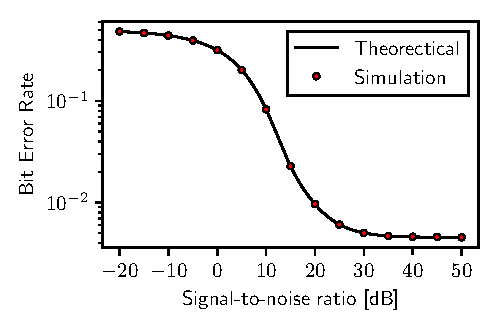
\includegraphics{figures/ber.eps}
    \caption{BER}
    \label{fig:ber}
\end{figure}

\section{Conclusions}

\bibliographystyle{IEEEtran}
\bibliography{manuscript.bib}

\end{document}
